\documentclass[conference]{IEEEtran}
\IEEEoverridecommandlockouts
% The preceding line is only needed to identify funding in the first footnote. If that is unneeded, please comment it out.
\usepackage{cite}
\usepackage{amsmath,amssymb,amsfonts}
\usepackage{algorithmic}
\usepackage{graphicx}
\usepackage{textcomp}
\usepackage{xcolor}
\usepackage{booktabs}
\def\BibTeX{{\rm B\kern-.05em{\sc i\kern-.025em b}\kern-.08em
    T\kern-.1667em\lower.7ex\hbox{E}\kern-.125emX}}
\begin{document}

\title{Mobile-PIRL: A Mobile Version of Self-Supervised Learning of Pretext-Invariant Representations\\
}

\author{\IEEEauthorblockN{İzzet Emre Küçükkaya}
\IEEEauthorblockA{
\textit{Boğaziçi University}\\
Istanbul, Turkey \\
izzet.kucukkaya@boun.edu.tr}
\and
\IEEEauthorblockN{Berkcan Üstün}
\IEEEauthorblockA{
\textit{Boğaziçi University}\\
Istanbul, Turkey \\
berkcan.ustun@boun.edu.tr}
}

\maketitle

\begin{abstract}
Supervised learning techniques of the Deep Neural Networks which are the main component of various applications in the domain of computer vision such as classification, segmentation or object detection are in need of the large amount of semantically annotated data in order to perform efficiently. However, it is a compelling situation to obtain a great quantity of semantically annotated data. The Self-Supervised learning techniques are introduced to overcome this obstacle. On the other hand, plenty of these techniques uses convolutional neural networks that have a great deal of complexity, parameters and inference time. In terms of performance, the recent mobile networks are considered to be comparable to complex network architectures despite their simple structure, few number parameters and less inference time. By this sense, the usage of newly introduced mobile networks in the domain of self supervised learning is an interesting topic of research. Regarding these facts, the performance of the mobile networks in a self supervised learning architecture can be examined. Our choice as the baseline architecture is PIRL (Pretext-Invariant Representation Learning). In addition, the number of transformations used in the PIRL can be increased along with the opportunity that they can be combined together.  
\end{abstract}

\begin{IEEEkeywords}
Mobile Networks, Data Augmentation, Self-Supervised Learning
\end{IEEEkeywords}

\section{Introduction}
Image representations are learned by modern image-recognition algorithms using massive datasets of photos and their semantic annotations. Class labels, hashtags, bounding boxes, and other types of annotations can be used to offer these annotations. Pre-defined semantic annotations do not scale well to the large tail of visual concepts, obstructing future image recognition advancements. Building more intelligent generalist models that can execute numerous applications and learn new abilities without vast quantities of labeled data is hampered by supervised learning. Self-supervised learning attempts to overcome these drawbacks by learning image representations from the pixels themselves rather than depending on those pre-defined lexical annotations. Many of the self-supervised learning techniques includes a pretext task which conducts a transformation to the input image with the need of the estimation of the properties of the transformation from the transformed image \cite{PIRL, Multitask,SimCLR,gidaris,zhangir}. 

\begin{figure}[h]
\centerline{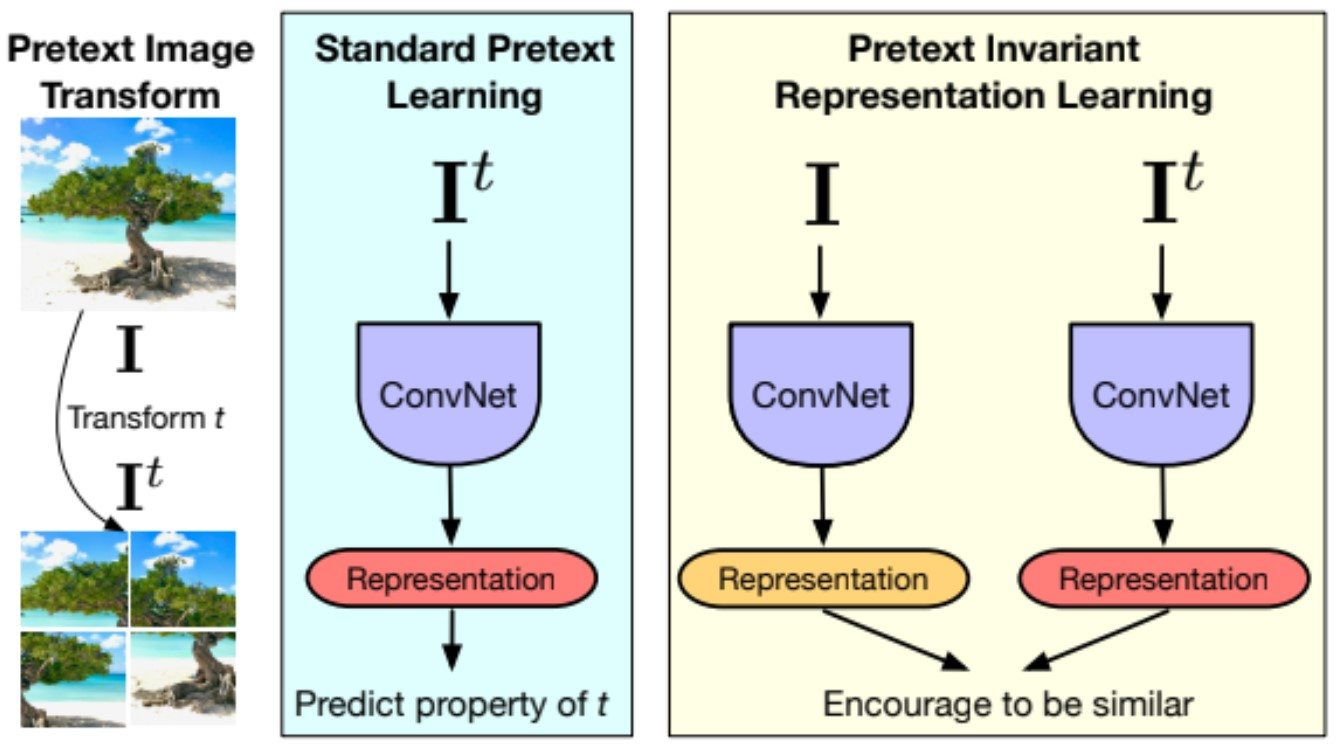
\includegraphics[width=8cm]{fig1.jpg}}
\caption{Comparison of the Standard Pretext Learning and Pretext Invariant Representation Learning \cite{PIRL}}
\label{fig}
\end{figure}

Although, often these techniques result on learning visual representations that are co-variant to the transformations, Pretext-Invariant Representation Learning (PIRL), which is one of the most successful methods, states the fact that learning co-variant representations is not useful for most of the visual recognition applications. In consideration of this, the PIRL underlines the necessity of learning invariant representations since the transformations do not change the semantics of the visual inputs. In order to obtain invariant representations, PIRL tries to create image representations that are close to other representations which are resulted in the transformation of the same image and far from the representations of other images.

PIRL uses primarily the "Jigsaw" pretext task which is based on the division of the input image to nine patches and shuffling them. In addition, rotation pretext task and the combination of those two tasks presented along with the Jigsaw. However, as mentioned in the original article \cite{PIRL}, the number of transformations can be enhanced in order to improve the performance. Bunch of transformations can be seen in the Figure \ref{fig2}. Those transformation can be engaged one by one, in the form of combination of two, three etc. 
\begin{figure*}[h]
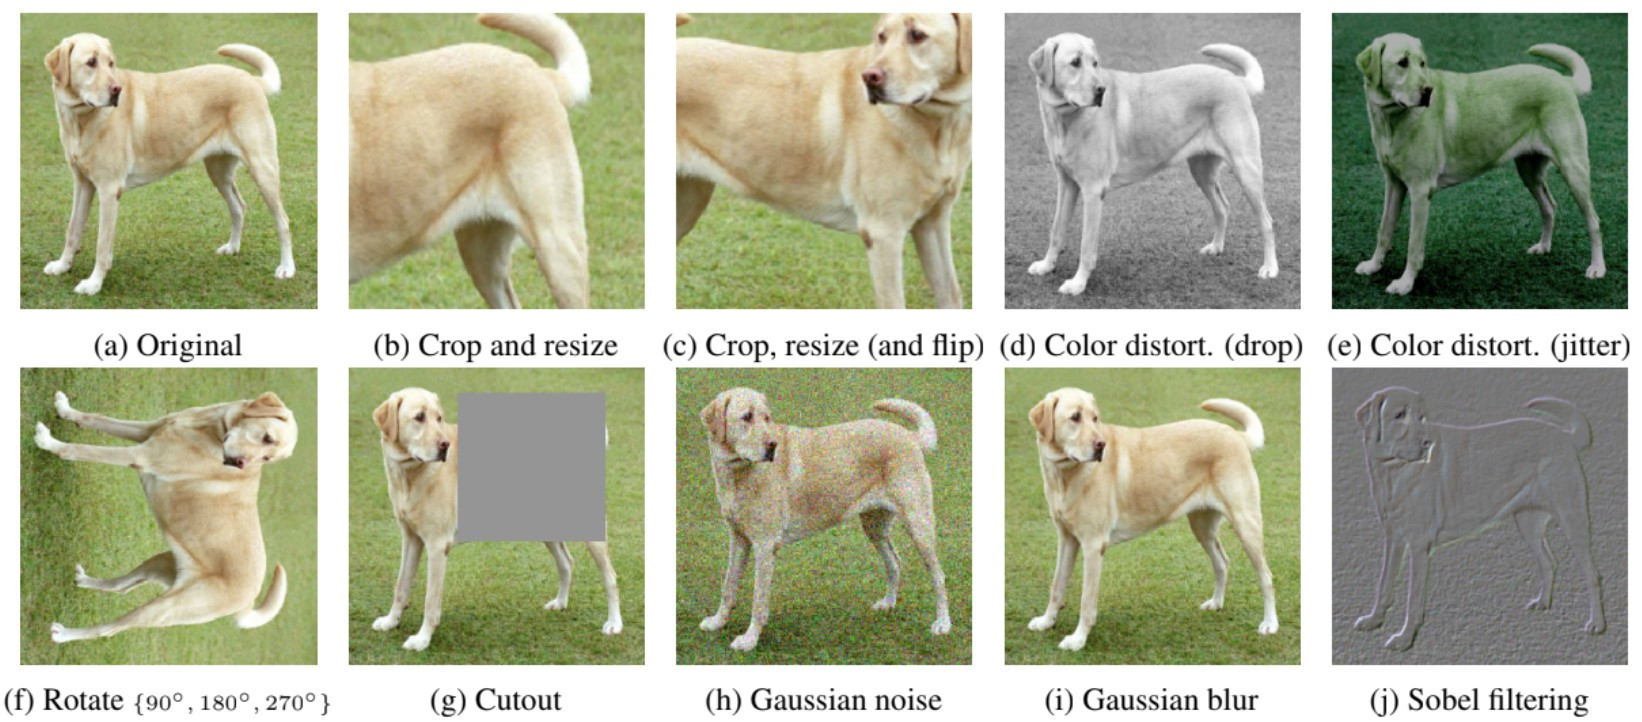
\includegraphics[width=\textwidth]{fig2.jpg}
\centering
\caption{Examples of data augmentations \cite{SimCLR}}
\label{fig2}
\end{figure*}

\begin{figure*}[h]
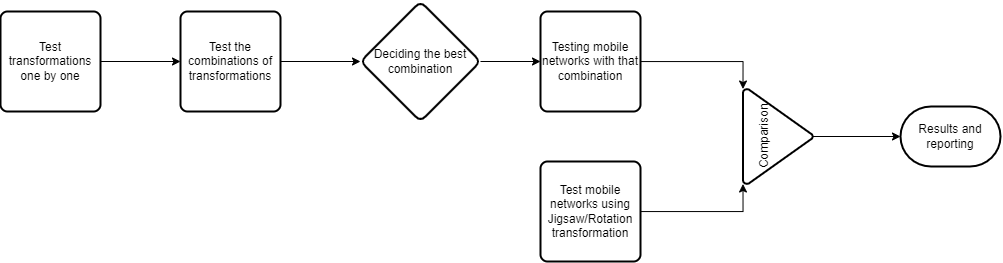
\includegraphics[width=\textwidth]{flowchartcmpe597.png}
\centering
\caption{Contingency Table}
\label{fig2}
\end{figure*}
PIRL uses the ResNet-50 \cite{resnet} architecture in order to obtain the image representations of both the original image and the transformed image. In spite of the fact that ResNet is an evolutionary architecture that accomplishes state-of-the-art performance with relatively small number of parameters and floating point operations, we think that there is still room for progress in the area of decreasing the parameters and floating point operations while keeping the performance at a some standard thanks to newly introduced concept mobile networks. The introduction of the mobile networks or so-called "Lightweight-CNNs" makes understand their efficacy in the real world applications such as augmented reality glasses. In real world applications, the problem of the memory usage can be arisen due to the great amount of parameters of the deep network architectures. Besides, the floating point operations and hence the inference of the standard very deep networks can be considerably grandiose giving rise to an obstacle to use these networks in the applications that the timing is essential. In consideration of these facts, various mobile networks has been constructed \cite{mnasnet,mobile2,efficientnet}. An example comparison of the mobile networks with the regular deep networks can be seen in the Table .. The table is taken from the original paper of the EfficientNet \cite{efficientnet}. As can be seen from the table, the EfficientNet-B0 structure overwhelms the other deep networks with only small number of parameters. As a result of this example comparison, it is a promising idea that mobile networks might be performing properly with fewer number of parameters in the domain of self-supervised learning.     

\begin{table*}
    \caption{
        \textbf{EfficientNet Performance Results on ImageNet \cite{efficientnet}} 
       }
  \vskip 0.1in
    \centering
    \resizebox{1.0\textwidth}{!}{
        \begin{tabular}{l|cc||cc||cc}
        \toprule[0.15em]
        Model &  Top-1 Acc. & Top-5 Acc. & \#Params &  Ratio-to-EfficientNet &\#FLOPs & Ratio-to-EfficientNet  \\
        \midrule[0.1em]
        \bf EfficientNet-B0  & \bf 77.1\% & \bf 93.3\% & \bf 5.3M  & \bf 1x & \bf 0.39B & \bf  1x \\
        ResNet-50 & 76.0\% & 93.0\% & 26M & 4.9x & 4.1B & 11x \\
        DenseNet-169 & 76.2\% & 93.2\% & 14M & 2.6x & 3.5B & 8.9x \\
        \bottomrule[0.15em]
        \multicolumn{7}{l}{}
        \end{tabular}
    }
    \label{tab:imagenet}
\end{table*}



\section{Proposed Approach}
Our proposed idea can be seen in the category of improving an already proposed idea since we are desiring to improve the Pretext-Invariant Representation Learning architecture by 1) increasing the number of transformations 2) changing ResNet-50 which is can be considered as the backbone of the architecture with various mobile networks. On the other hand, since the performance of the mobile networks have never been examined in the self-supervised learning architectures, this work might be considered as applying an already proposed method to a different domain.  

\subsection{Mobile Networks with Jigsaw Transformation}\label{AA}
The first thing to do is the test the performance of the mobile networks. In order to create the controlled experiment environment, the mobile networks must be integrated to the PIRL with the Jigsaw pretext task same as the \cite{PIRL}. The same experiments must be conducted in order to get a healthy comparison of the mobile networks with the ResNet \cite{resnet} in the self-supervised learning.

\subsection{Deciding the Best Combination of Transformations}
In order to decide the best combination of the transformations, various combinations of the transformations must be tried with the same network. This network can be the ResNet itself or it can be the best performing mobile network. 

\subsection{Mobile Networks with the Best Transformation}
In this part, the best transformation can be examined with the mobile networks. 


\subsection{Overall}\label{SCM}
The best transformation combination-mobile network duo is going to be tried to find. The number of transformations and the number of mobile networks are not be determined yet. Given the fact that training convolutional neural networks takes time, those numbers must be chosen efficiently.

\bibliographystyle{IEEEtran}
\bibliography{sample}
\vspace{12pt}

\end{document}